%--------------------------------------------------------------------------------
%\documentclass{article}

\documentclass[12pt]{article}
\usepackage[T1]{fontenc} 
\usepackage[bf]{caption}
\usepackage{hyperref}
\usepackage[all]{hypcap}
\usepackage[utf8]{inputenc}
\usepackage{graphicx}
\usepackage[czech, english]{babel}
\selectlanguage{czech}
\usepackage{subfig}                % \subfloat
\usepackage{color}
\usepackage{url}
\inputencoding{utf8}
%\usepackage[bf]{caption2}
\usepackage{hyperref}
\usepackage[all]{hypcap}
\hypersetup{colorlinks=false, linkbordercolor=1 1 1, citebordercolor=1 1 1}
\usepackage[right]{lineno}
\renewcommand\linenumberfont{\normalfont\tiny\color{blue}}


\title{Sledování objektu v obraze s využitím částicového filtru}
\author{Jan Hamrský <xhamrs00@stud.fit.vutbr.cz> \\
        Václav Maliňák <xmalin19@stud.fit.vutbr.cz> \\
        Jan Wozniak <xwozni00@fit.vutbr.cz>}
\date{\today}


%--------------------------------------------------------------------------------


\begin{document}
\selectlanguage{czech}
\maketitle

\section{Úvod}

Cílem našeho projektu bylo vytvořit aplikaci schopnou sledovat pohybující se objekt v obraze pomocí částicového filtru, v našem případě varianty CONDENSATION algoritmu, a tu aplikovat na zvolenou
úlohu. Jako tu jsme si vybrali sledování aut na cestě\footnote{jako data byly použity videa z projektu \url{http://www.eecs.qmul.ac.uk/~andrea/avss2007\_d.html}}. Uživatel aplikace označí v rámci videosekvence oblast, kde se nachází objekt zájmu a aplikace tento objekt sleduje a vizuálně jej označí. Příznaky extrahované z obrazu byly použity HSV histogram, LBP histogram a BRIEF.

%%%%%%%%%%%%%%%%%%%%%%%%%%%%%%%%%%%%%%%%%%%%%%%%%%%%%%%%%%%%%%%%%%%%%%%%%%%%%%%%%%%%%%%%

\section{Teorie}

\subsection*{Particle filter}
Cílem částicového filtru je odhadnutí stavových proměnných popisující sle-
dovaný objekt na základě naměřených hodnot z dat. Samotné částicové fil-
trování pak znamená, že je aproximována distribuční funkce neznámých pro-
měnných pomocí částic, které reprezentují různě váhované vzorky distribuční
funkce.

CONDENSATION algoritmus (\cite{isard98}) se skládá z několika kroků, které jsou cyk-
licky opakovány po dobu běhu trasování. V každém z nich je na konci kroku
k dispozici aproximovaný stav objektu.

První krok, který je teoreticky volán pouze jednou, je inicializační
krok, ve kterém je inicializován model objektu a částice
s uniformní pravděpodobností. V našem programu je inicializace prováděna
vždy při ručním znovunainicializování uživatelem pomocí GUI.

Stejně tak jako v původním CONDENSATION algoritmu je i naše částice
ve tvaru $(sn , \pi_n, c_n )$, kde $s_n$ je prvek stavového prostoru, $\pi_n$ pravděpodobnost
částice a $c_n$ kumulativní pravděpodobnost.

\subsubsection*{Resampling}
  V kroku vzorkování jsou vybrány částice, které nezaniknou a budou distribuovány
  do dalších kroků algoritmu. Tyto částice vybíráme na základě jejich kumulativní 
  pravděpodobnosti (rostoucí posloupnost čísel s $\pi_n$) a náhodně generovaného čísla
  $r$ s uniformním rozložením.

\subsubsection*{Dynamický model}
  Dynamický model určuje způsob, jakým se mění stav částice mezi jednotlivými kroky.
  Často používanými modely jsou autoregresivní rovnice prvního a druhého řádu, která 
  je určena rovnicí 
  $$X_{n} = A_0 * X_{n-1} + A_1 * X_{n-2} + B * w$$
  kde $X_n$ je stav objektu v čase $n$, $A_0$,$A_1$, $B$ jsou koeficienty určující 
  dynamiku modelu a $w$ je vektor náhodných standartních normálních proměnných.
  Takto zapsaná rovnice určuje tzv. \uv{deterministický drift} a Brownovské pohyby
  (zašumění).
  
\subsubsection*{Observační model}
  Observační model určuje pravděpodobnost částice. Naším vybraným modelem je 
  $$p(z_t | x_t = s_t) = e^{-\kappa * D[h_0, h_t]}$$
  kde $D$ je metrikou na histogramech (euclidova vzdálenost, Bhattacharya, $\chi$-kvadrát, \ldots).
  Koeficient $\kappa$ lze určit z dat pomocí MLE, ale touto možností jsme se nezabývali.

\subsubsection*{Odhad}
  Na konci každého kroku je možné provést odhad stavu, který je váhovanou sumou 
  stavů částic a dostat tak \uv{průměrnou hodnotu}.


\subsection*{Příznaky}
Z obrazu jsou extrahovány příznaky pro přesnější sledování objektu. HSV histogram funguje velmi spolehlivě pro barevný obraz avšak nedokáže si poradit s problémem, kdy naprosto odlišný objekt má  podobné rozložení barevných složek a proto jsme se rozhodli najít jiný vhodný příznak, který by byl výpočetně nenáročný a reprezentoval by do jisté míry i strukturu hledaného objektu. 

Textura oblasti v obraze může v daném problému sloužit jako velmi základní popis reflektující rovněž strukturu objektu, proto jsme se pokusili použít LBP histogram\cite{lbp}. Zkoušeli jsme dvě varianty LBP(8,1) rotačně invariantní a LBP(8,1) uniformní, a metriky $\chi^2$, L1, euklidovskou a Bhattacharya. Nejlepší výsledky podávaly uniformní LBP s metrikou L1.

BRIEF\cite{brief} je obvykle používán jako deskriptor významných bodů v obraze pracující na principu náhodně vybraných porovnání dvojic bodů v okně pevné velikosti. Testovali jsme základní variantu s uniformním rozložením lokace bodů $(x_i, y_i)$, tedy $(-\frac{S}{2}, \frac{S}{2})$. Metriku pro BRIEF jsme použili Hammingovu.



%%%%%%%%%%%%%%%%%%%%%%%%%%%%%%%%%%%%%%%%%%%%%%%%%%%%%%%%%%%%%%%%%%%%%%%%%%%%%%%%%%%%%%%%

\section{Vyhodnocení}

Pro výběr vhodných příznaků jsme si vytvořili databázi, na které jsme se změřili diskriminabilitu hledaných objektů pomocí turnajové selekce. Cílem našeho projektu bylo sledovat jedoucí automobil v záznamu z kamery na základě výběru uživatele.

\begin{figure}[htb]
  \centering
  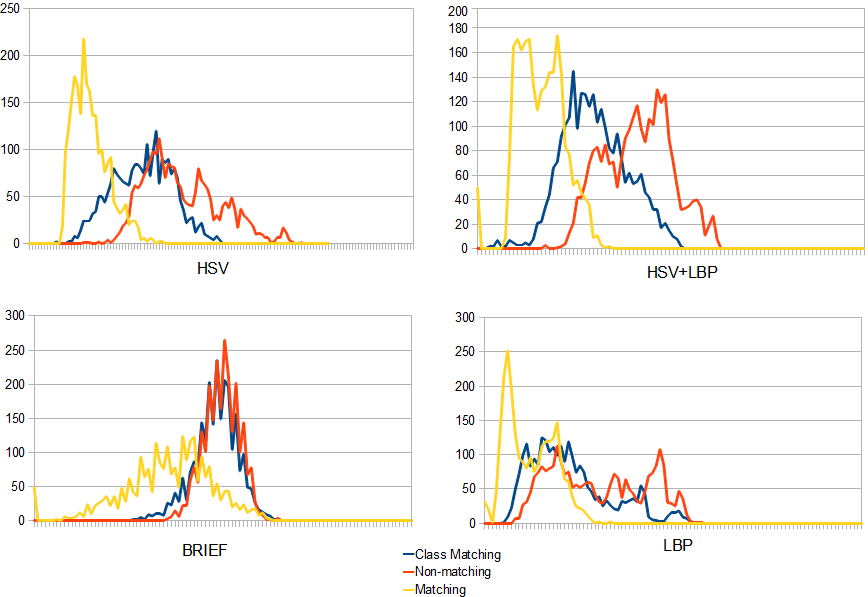
\includegraphics[scale=0.60]{all.png}
  \caption{Graf distribuce vzdáleností.}
  \label{graph}
\end{figure}
Na každém grafu z obrázku \ref{graph} jsou tři distribuční křivky, žlutá znázorňuje rozložení vzdáleností mezi příznaky hledaného objektu (obrázky konkrétního vozu), modrá mezi objektem a třídou těchto objektů (obrázky různých vozů), červená mezi objektem a okolím. Jak je z grafů patrné, LBP a HSV byly úspěšnější než BRIEF, proto jsme se pokusili spojit LBP a HSV. Podle distribuce by toto spojení mělo přinést zlepšení.

Pokusili jsme se naimplementovat algoritmus CONDENSATION. Kroky jsme implementovali stejně tak, jako byly popsány v článku. Jako stav objektu jsme zvolili $\left[x,y\right]$. V rámci projektu jsme se také pokusili stanovit koeficienty dynamického modelu na základě článku \cite{blake95}. S pomocí programu \textit{ViPER}\footnote{\url{http://viper-toolkit.sourceforge.net/}} jsme provedli určení \textit{ground truth}. Kvůli námi nezjištěné chybě v programu nebylo možné získané koeficienty použít, protože chyba znemožňovala použití autoregresivní rovnice 2. řádu.

O stanovení koeficientu $\kappa$ jsme se nepokoušeli.
%%%%%%%%%%%%%%%%%%%%%%%%%%%%%%%%%%%%%%%%%%%%%%%%%%%%%%%%%%%%%%%%%%%%%%%%%%%%%%%%%%%%%%%%

\section{Závěr}
HSV příznaky i LBP příznaky samy o sobě by měly rozlišit objekt od okolí. Spojením těchto dvou příznaků bychom měli dosáhnout zlepšení diskriminačních vlastností, to se nám ale v částicovém filtru z časových důvodů nepodařilo ověřit.

Algoritmus CONDENSATION je poměrně efektivní způsob pro sledování objektu v obraze, který funguje v téměř reálném čase v závislosti na velikosti inicializační oblasti a použitých příznacích. V rámci projektu se nám podařilo vytvořit sledování objektu na základě šumového modelu, ne však s použitím autoregresivní funkce 2. řádu. Původně zamýšlenou metriku překrytí detekovaných ploch s ground truth nebylo možné použít kvůli již uvedeným problémům.
\bibliographystyle{alpha}
\begin{flushleft}
  \bibliography{project}
\end{flushleft}

%\appendix
%\newpage
%\section{}

\end{document}
